\documentclass{article}

% Required packages
\usepackage{amssymb}
\usepackage{amsmath}
\usepackage{graphicx}
\usepackage{geometry}
\usepackage{tikz}
\usepackage{array}
\usepackage{booktabs}
\usepackage{enumitem}
\usepackage{listings}
\usepackage{xcolor}
\usepackage{fancyhdr}
\usepackage{float}
\usepackage{subcaption}

% Set page geometry
\geometry{a4paper, margin=1in}

% Configure listings for Python
\lstset{
  language=Python,
  basicstyle=\ttfamily\footnotesize,
  numbers=left,
  numberstyle=\tiny\color{gray},
  frame=single,
  breaklines=true,
  breakatwhitespace=true,
  captionpos=b,
  tabsize=4,
  showspaces=false,
  showstringspaces=false,
  showtabs=false,
  commentstyle=\color{gray}\textit,
  keywordstyle=\color{blue}\bfseries,
  stringstyle=\color{red}
}

\begin{document}

\pagestyle{fancy}
\chead{DSC 255: Machine Learning Fundamentals (Spring 2025)}
\lhead{Homework 8}
\rhead{Randall Rogers}

\subsection*{Solution 1}
\noindent\rule{\textwidth}{0.4pt}\\

\subsubsection*{Step 1}
\parbox{\textwidth}{
Rearrange the decision boundary equation to match the form $w \cdot \Phi(x) + b = 0$.

$$x_{1} + 3 x_{1} x_{2} = 6 x_{2}^{2} + 8 \hspace{0.5cm} \rightarrow  \hspace{0.5cm} x_{1} + 3 x_{1} x_{2} - 6 x_{2}^{2} - 8 = 0$$

}

\subsubsection*{Step 2}
\parbox{\textwidth}{
Identify the coefficients that correspond to each component of the basis expansion $\Phi(x) = \left(x_{1}, x_{2}, x_{1}^{2}, x_{2}^{2}, x_{1} x_{2}\right)$.
\begin{center}
  \begin{align*}
    0 =& w_1 x_{1} + w_2 x_{2} + w_3x^{2}_{1} + w_4x^{2}_{2} + w_5 x_{1} x_{2} + b& \\
    0 =& (1) x_{1} + (0)x_{2} + (0)x^{2}_{1} - 6 x_{2}^{2} + 3 x_{1} x_{2} - 8& 
  \end{align*}
\end{center}

It follows that each element of the weight vector is:
\begin{align*}
w_1 &= 1\\
w_2 &= 0 \\
w_3 &= 0 \\
w_4 &= -6\\
w_5 &= 3
\end{align*}
}

\subsubsection*{\normalfont}{$\therefore$ The weight vector is $w = (1, 0, 0, -6, 3)$}

\noindent\rule{\textwidth}{0.4pt}\\

\newpage

\subsection*{Solution 2 (a)}
\noindent\rule{\textwidth}{0.4pt}\\

\subsubsection*{Step 1}
\parbox{\textwidth}{
The dimension of $\Phi(x)$, is just the sum of the number of components in the expanded feature vector.

Given:
$$\Phi(x) = \left(x_{1}, \ldots, x_{4}, x_{1}^{2}, \ldots, x_{4}^{2}, x_{1} x_{2}, \ldots, x_{3} x_{4}\right)$$

Each type of term has the following number of elements:
\begin{itemize}
    \item Original features ($t_1$): $x_1, x_2, x_3, x_4$ (4 terms)
    \item Squared terms ($t_2$): $x_1^2, x_2^2, x_3^2, x_4^2$ (4 terms)
    \item Cross-product terms ($t_3$): $x_1x_2, x_1x_3, x_1x_4, x_2x_3, x_2x_4, x_3x_4$ (6 terms)
\end{itemize}

$$dim(\Phi(x)) = t_1 + t_2 + t_3 = 4 + 4 + 6 = 14 $$
}

\subsubsection*{\normalfont}{$\therefore$ The dimension of $\Phi(x)$ is 14.}

\noindent\rule{\textwidth}{0.4pt}\\

\newpage

\subsection*{Solution 2 (b)}
\noindent\rule{\textwidth}{0.4pt}\\

\subsubsection*{Step 1}
\parbox{\textwidth}{
The decision boundary of the Perceptron has the form:
$$w \cdot \Phi(x) + b = 0$$


}

\subsubsection*{Step 2}
\parbox{\textwidth}{
Now, expand the dot product of the decision boundary.
$$w_1 x_{1} + \ldots+ w_4 x_{4} + w_5 x_{1}^{2}+ \ldots + w_{14} x_{3} x_{4}$$
From \textbf{Solution 2 (a)} we know that the dimension of $\Phi(x)$ is 14, and  it follows that the weight vector $w$ must also have 14 components to match each feature in the expanded space.
}

\subsubsection*{\normalfont}{$\therefore$ The dimension of $w$ is 14.}

\noindent\rule{\textwidth}{0.4pt}\\

\newpage

\subsection*{Solution 3 (a)}
\noindent\rule{\textwidth}{0.4pt}\\

\subsubsection*{Step 1}
\parbox{\textwidth}{
When we map to the expanded feature space via $\Phi(x)$, we preserve the linear separability of the dataset. This is because:
\begin{itemize}
  \item If a dataset is separable in a space $\mathbb{R}^d$, it remains separable when mapped to a higher-dimensional space $\mathbb{R}^{D}$ where $D > d$.
  \item The new space actually provides additional flexibility for finding a separating hyperplane. The original linear separator can be represented in the expanded space by setting the weights for all quadratic terms to zero and keeping the weights for the linear terms as they were in the original space.
\end{itemize}
Hence, when we apply the basis expansion $\Phi(x)$ to our linearly separable dataset, we preserve the linear separability of the dataset. According to the Perceptron convergence theorem, the algorithm will converge in a finite number of steps.
}

\subsubsection*{\normalfont}{$\therefore$ The Perceptron algorithm will converge when using the given basis expansion on a linearly separable dataset.}

\noindent\rule{\textwidth}{0.4pt}\\

\newpage

\subsection*{Solution 3 (b)}
\noindent\rule{\textwidth}{0.4pt}\\

\subsubsection*{Step 1}
\parbox{\textwidth}{
We are given:
\begin{enumerate}
\item The original dataset is linearly separable in $\mathbb{R}^d$.
\item This means there exists at least one solution using only the original features (i.e., a solution where quadratic term weights are zero).
\item However, in the expanded feature space, there can be many other separating hyperplanes that use the quadratic terms.
\end{enumerate}
}
\subsubsection*{Step 2}
\parbox{\textwidth}{
\textit{Note: The Perceptron algorithm does not optimize for having zero weights in particular dimensions, it simply tries to find any separating hyperplane.}\\

The final weight vector depends on:
\begin{itemize}
\item The initialization of the weights
\item The order in which training examples are presented
\item The number of updates made during training
\end{itemize}
Hence, the Perceptron has no inherent bias toward solutions with zero weights for the quadratic terms.\\

\textit{Note: There is no guarantee that it will find such a solution, even though such a solution could exist.}
}

\subsubsection*{\normalfont}{$\therefore$ The Perceptron algorithm will not necessarily return a weight vector $w$ in which the entries corresponding to quadratic terms in $\Phi(x)$ are zero.}

\noindent\rule{\textwidth}{0.4pt}\\

\newpage


\subsection*{Solution 4 (a)}
\noindent\rule{\textwidth}{0.4pt}\\

\subsubsection*{Step 1}
\parbox{\textwidth}{
  There are five updates in the following order:
  \begin{itemize}
      \item Zero updates on point $x^{(1)}$ (label +1)
      \item Two updates on point $x^{(2)}$ (label +1)
      \item Two updates on point $x^{(3)}$ (label -1)
      \item One update on point $x^{(4)}$ (label -1)
  \end{itemize}
\textit{Note: $\alpha = (\alpha^{(1)},\alpha^{(2)},\alpha^{(3)}\alpha^{(4)})$, where $\alpha^{(i)} = \alpha^{(i)} + 1$ when the point is misclassified.}
}

\subsubsection*{Step 2}
\parbox{\textwidth}{
Calculate $\alpha^{(i)}$ for each point.
}

$$\alpha^{(1)} = \alpha^{(1)} + 1 = \text{updates}_1 = 0 $$
$$\alpha^{(2)} = \alpha^{(2)} + 1 = \text{updates}_2 = 2$$
$$\alpha^{(3)} = \alpha^{(3)} + 1 = \text{updates}_3 = 2$$
$$\alpha^{(4)} = \alpha^{(4)} + 1 = \text{updates}_4 = 1$$

\subsubsection*{\normalfont}{$\therefore$ The final value of $\alpha$ is $(0, 2, 2, 1)$.}

\newpage

\noindent\rule{\textwidth}{0.4pt}\\

\subsection*{Solution 4 (b)}
\noindent\rule{\textwidth}{0.4pt}\\

\subsubsection*{Step 1}
\parbox{\textwidth}{
  There are five updates in the following order:
  \begin{itemize}
      \item Zero updates on point $x^{(1)}$ (label +1)
      \item Two updates on point $x^{(2)}$ (label +1)
      \item Two updates on point $x^{(3)}$ (label -1)
      \item One update on point $x^{(4)}$ (label -1)
  \end{itemize}
\textit{Note: $b= b^{(1)}+b^{(2)}+b^{(3)}+b^{(4)}$, where $b^{(i)} = b^{(i)} + y^{(i)}$ when the point is misclassified.}
}

\subsubsection*{Step 2}
\parbox{\textwidth}{
Calculate $b^{(i)}$ for each point and find sum.
}

$$b^{(1)} = b^{(1)} + y^{(1)} = \text{updates}_n \cdot \text{label} = 0 \cdot 1 = 0$$
$$b^{(2)} = b^{(2)} + y^{(2)} = \text{updates}_n \cdot \text{label} = 2 \cdot 1 = 2$$
$$b^{(3)} = b^{(3)} + y^{(3)} = \text{updates}_n \cdot \text{label} = 2 \cdot -1 = -2$$
$$b^{(4)} = b^{(4)} + y^{(4)} = \text{updates}_n \cdot \text{label} = 1 \cdot -1 = -1$$
$$b = b^{(1)} + b^{(2)} + b^{(3)} + b^{(4)} = 0 + 2 + (-2) + (-1) = -1$$

\subsubsection*{\normalfont}{$\therefore$ The final value of $b$ is $-1$.}

\newpage

\subsection*{Solution 5 (a)}
\noindent\rule{\textwidth}{0.4pt}\\

\subsubsection*{Step 1}
\parbox{\textwidth}{
The vector $\alpha$ corresponds to the number of training points. 
In the example from class we have 18 red circles and 18 black triangles, for a total of 36 training points.
}

\subsubsection*{\normalfont}{$\therefore$ The dimension of $\alpha$ is 36.}

\noindent\rule{\textwidth}{0.4pt}\\

\newpage



\subsection*{Solution 5 (b)}
\noindent\rule{\textwidth}{0.4pt}\\

\subsubsection*{Step 1}
\parbox{\textwidth}{
The condition $\alpha_i > 0$ is simply the count of support vectors for the SVM and we have 6 support vectors in the example from class.
}
\subsubsection*{\normalfont}{$\therefore$ There are 6 entries in $\alpha$ that are $> 0$.}

\noindent\rule{\textwidth}{0.4pt}\\

\newpage

\subsection*{Solution 5 (c)}
\noindent\rule{\textwidth}{0.4pt}\\

\subsubsection*{Step 1}
\parbox{\textwidth}{
For a kernel SVM, $\alpha_i$ is subject to the following constraint:

$$0 \leq \alpha_i \leq C \quad \forall i$$
}

\subsubsection*{\normalfont}{$\therefore$ There are 0 entries in $\alpha$ that are $< 0$.}

\noindent\rule{\textwidth}{0.4pt}\\

\newpage

\subsection*{Solution 5 (d)}
\noindent\rule{\textwidth}{0.4pt}\\

\subsubsection*{Step 1}
\parbox{\textwidth}{
We have 2 support vectors for the black triangle class and 4 support vectors for the red circle class.
The resulting SVM has to optimize the margin more for the red circles and leads to a larger green margin.
}

\subsubsection*{\normalfont}{$\therefore$ The imbalance of support vectors between the classes leads to a larger green margin.}

\noindent\rule{\textwidth}{0.4pt}\\

\newpage

\subsection*{Solution 6}
\noindent\rule{\textwidth}{0.4pt}\\

\subsubsection*{Python Code}
\begin{lstlisting}
def quadratic_kernel(x, z, c):
    return (np.dot(x, z) + c)**2

def rbf_kernel(x, z, c):
    return np.exp(-np.linalg.norm(x-z)**2/(2*c**2))

def train(x, y, kernel_function, c=1.0, max_iter=1000):
    n_samples = len(x)
    alpha = np.zeros(n_samples)
    b = 0
    
    ## calculate kernel matrix before looping through dataset
    K = np.zeros((n_samples, n_samples))
    for i in range(n_samples):
        for j in range(n_samples):
            K[i, j] = kernel_function(x[i], x[j], c)
    
    ## training loop for max iterations
    for _ in range(max_iter):
        mistakes = False    
        for i in range(n_samples):
            ## calculate predicted label
            f_xi = 0
            for j in range(n_samples):
                f_xi += alpha[j] * y[j] * K[i, j]
            f_xi += b           
            ## update b and alpha if prediction is wrong
            if y[i] * f_xi <= 0:
                alpha[i] += 1
                b += y[i]
                mistakes = True        
        ## stop training loop if all predictions are correct
        if not mistakes:
            print("converged!")
            break
    return alpha, b

def classify(x, y, alpha, b, xi, kernel_function, c=1.0):
    f_xi = 0
    for i in range(len(x)):
        f_xi += alpha[i] * y[i] * kernel_function(x[i], xi, c)
    f_xi += b
    return 1 if f_xi >= 0 else -1

\end{lstlisting}
\newpage

\subsubsection*{Plots}
\begin{figure}
  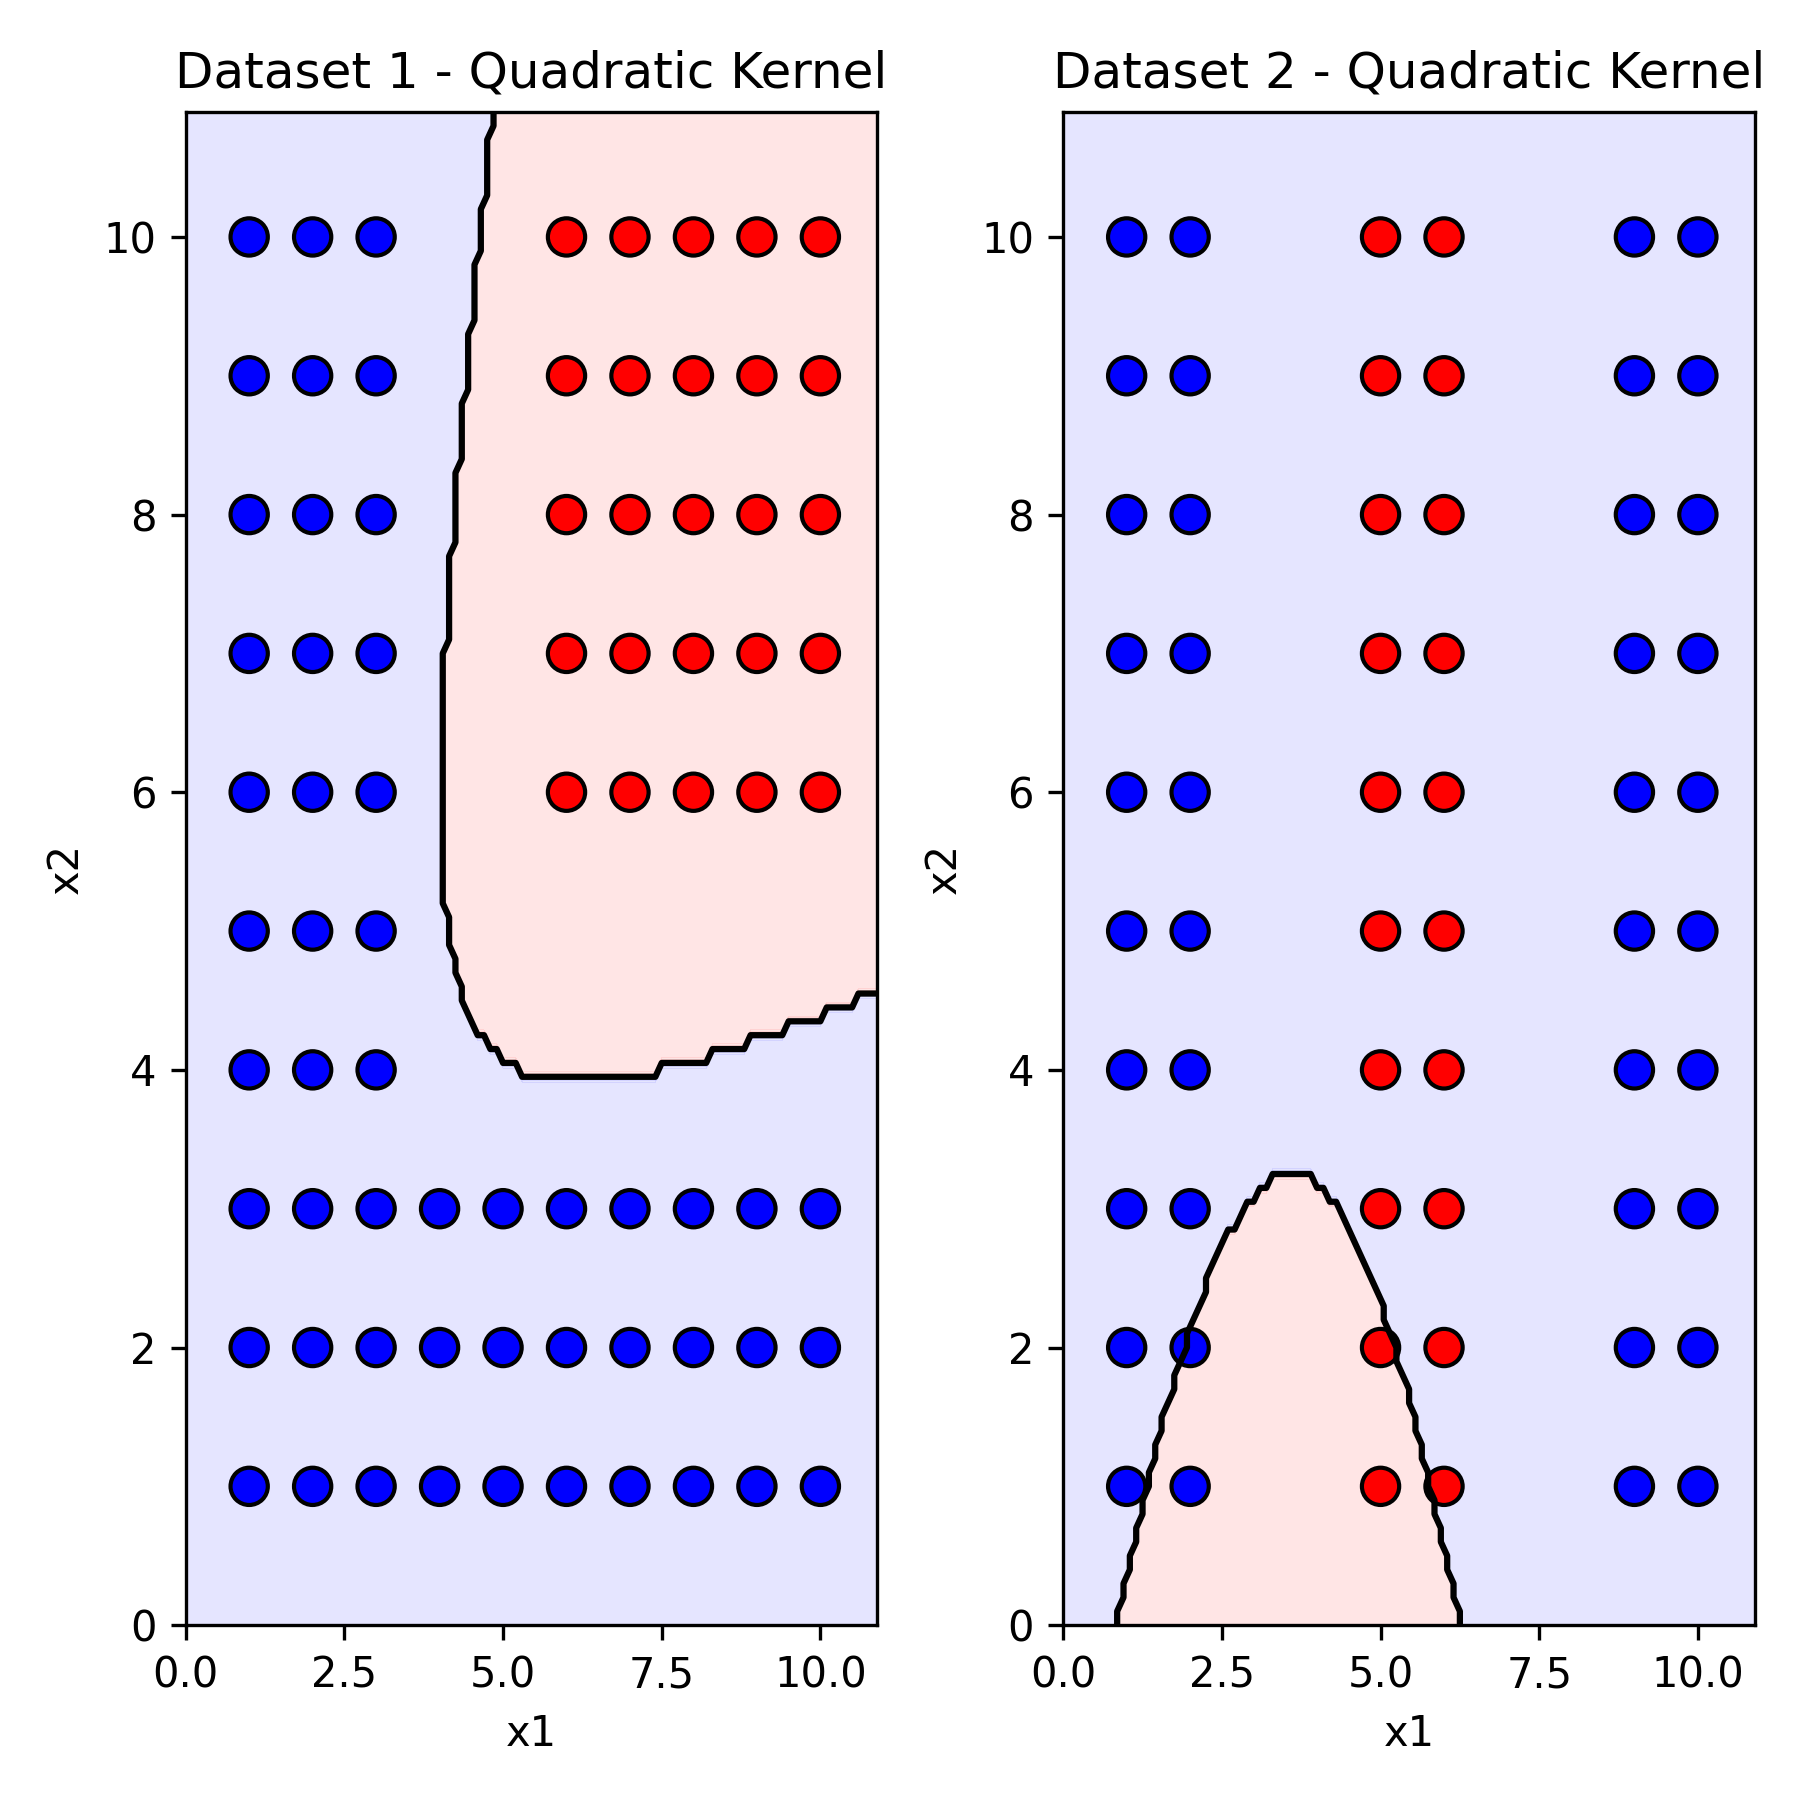
\includegraphics{part_a_quadratic_kernel.png}
  \caption{Decision boundary for quadratic kernel}
\end{figure}

\begin{figure}
  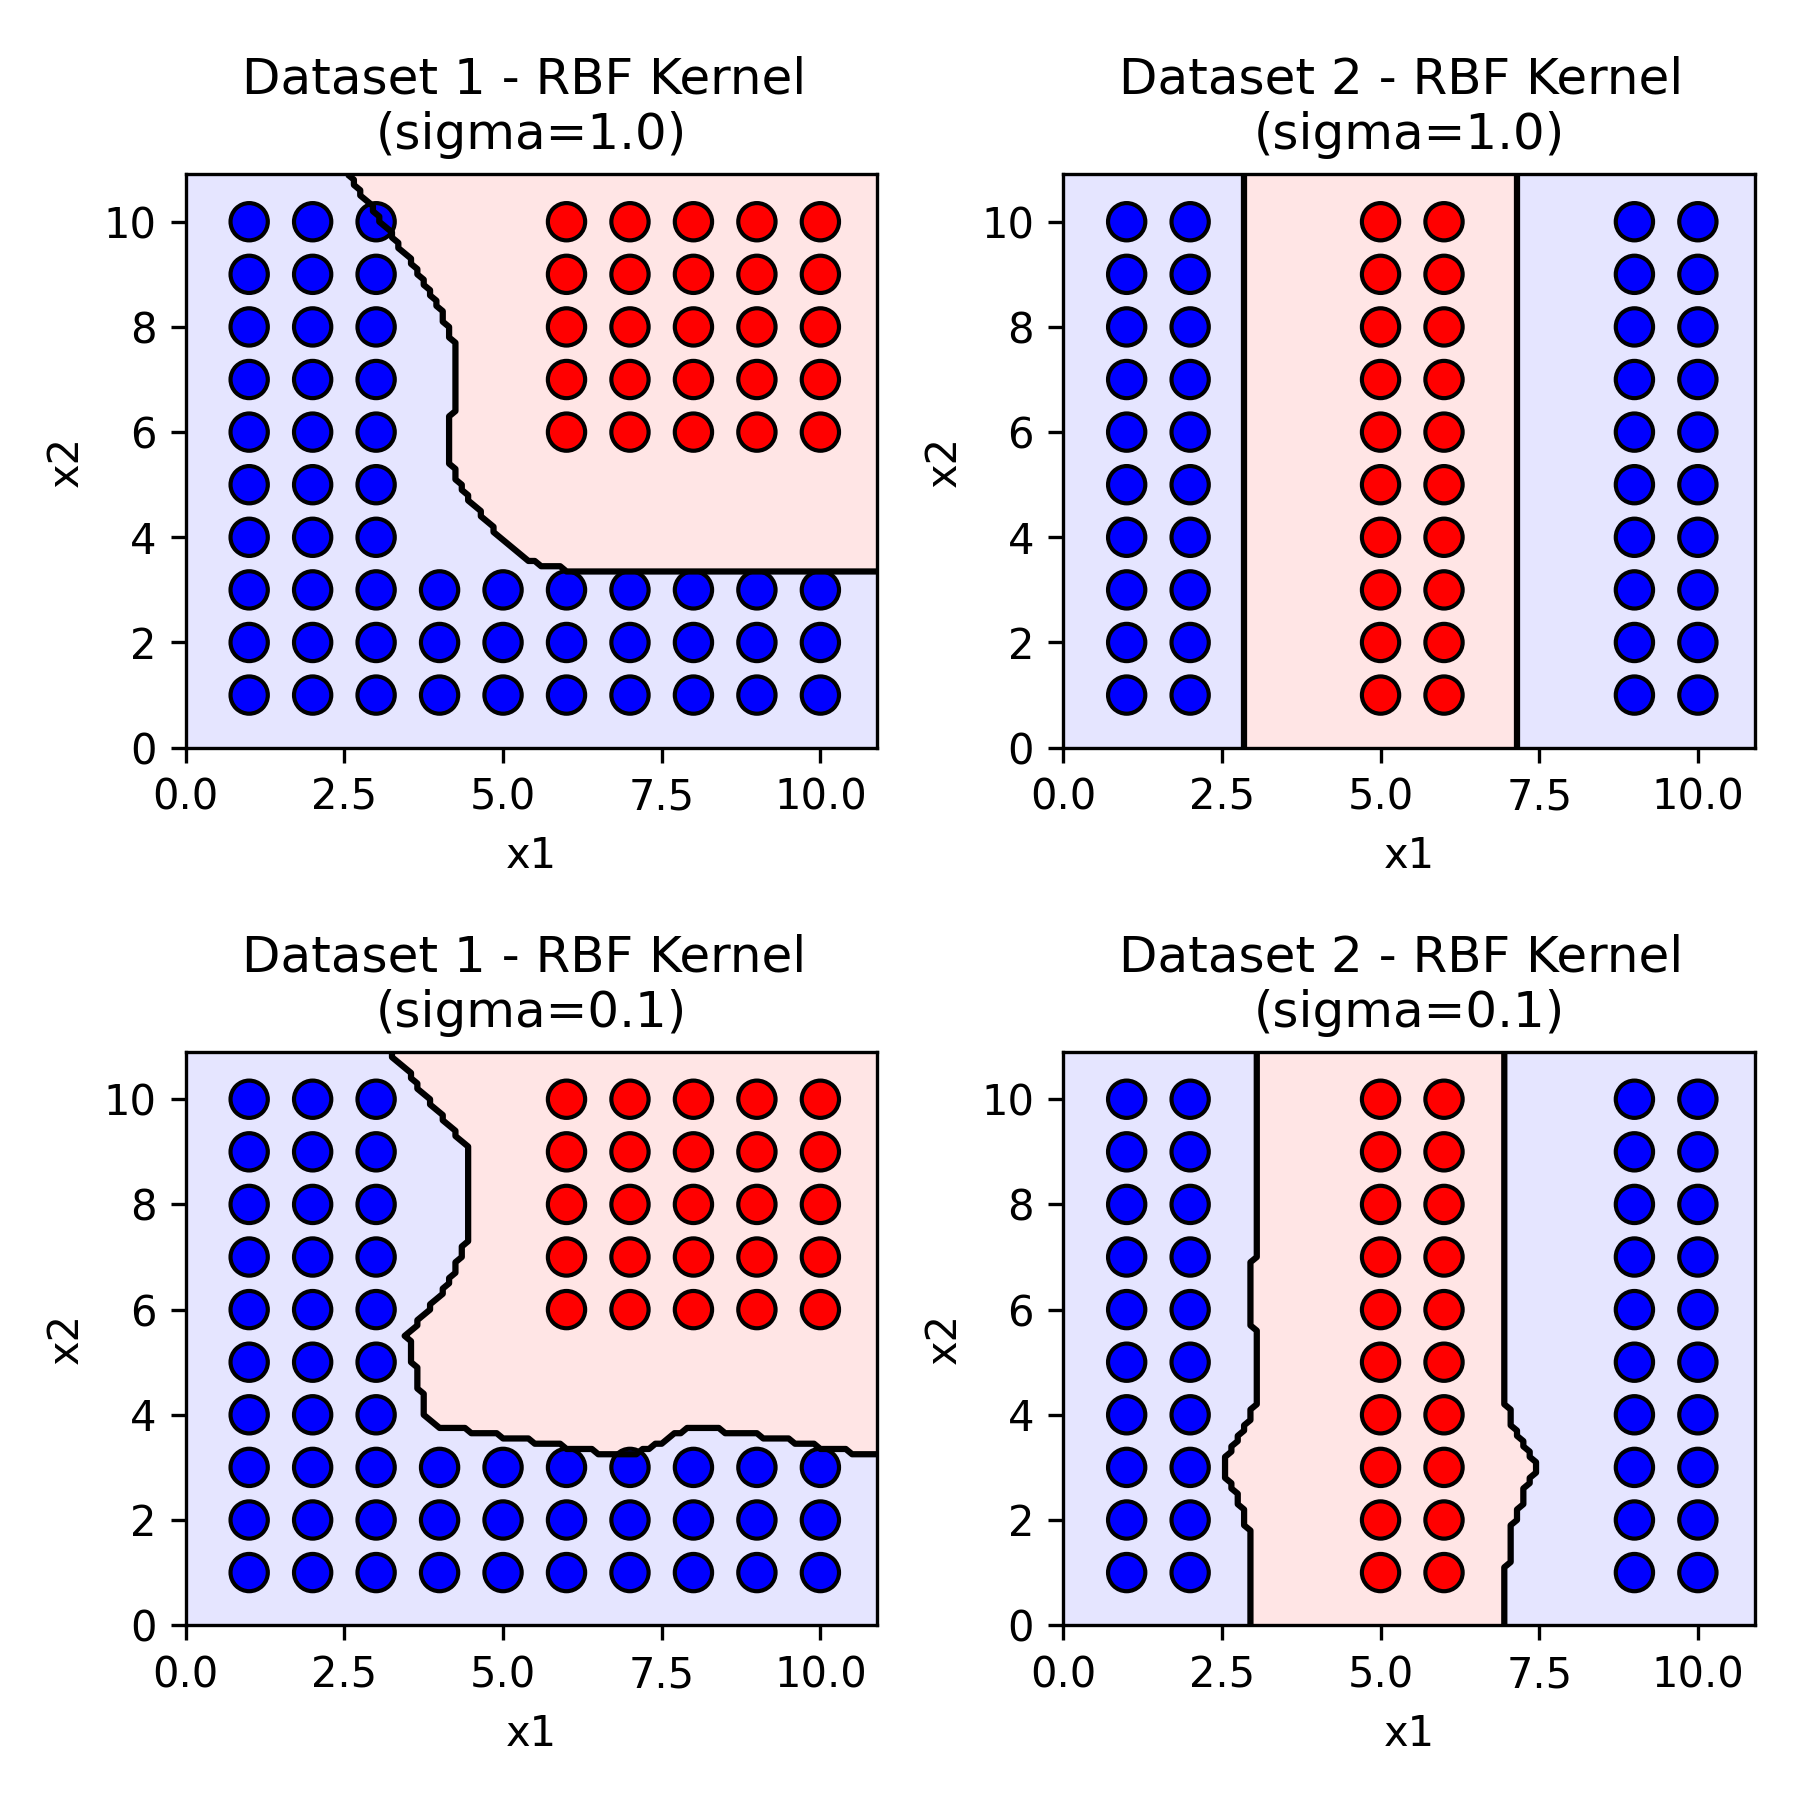
\includegraphics{part_b_rbf_kernel.png}
  \caption{Decision boundary for rbf kernel}
\end{figure}
\noindent\rule{\textwidth}{0.4pt}\\

\newpage

\subsection*{Solution 7}
\noindent\rule{\textwidth}{0.4pt}\\

\subsubsection*{Linear SVM}

\begin{center} 
  \begin{tabular}{|c|c|c|} 
    \hline C Value & Training Error (\%) & Test Error (\%) \\ 
    \hline 
    0.01 & 16.32 & 15.48\\ 
    0.1 & 15.91 & 16.36 \\
    1.0 & 14.25 & 14.04 \\
    10.0 & 13.56 & 13.16 \\ 
    100.0 & 14.05 & 14.78 \\ 
    \hline
  \end{tabular}
\end{center}
\parbox{\textwidth}{Based on the results above it seems that the data is linearly separable.}
\subsubsection*{Quadardic SVM}
\begin{center} 
  \begin{tabular}{|c|c|c|} 
    \hline Training Error (\%) & Test Error (\%)  & Support Vectors\\ 
    \hline 
    0.17 & 2.13 & 17906\\ 
    \hline
  \end{tabular}
\end{center}

\end{document}

